\chapter{Analysis}
\label{chapter:analysis}

\section{Uncertainties}
\label{sec:uncertainties}

\subsection{Statistical Uncertainties}
\label{ssec:stat_uncertainty}

The statistical uncertainties due to the number of data events are propagated
through the unfolding method, as discussed in
\SEC~\ref{ssec:unfolding_statistical_uncertainties}. This uncertainty is
ranges from 0.3 to 1.2\% for both the absolute and normalized cross section
measurement. It is one of the dominant uncertainties for the normalized cross
section measurement.

\subsection{Statistical Uncertainties from the Monte Carlo Samples}
\label{ssec:mc_stat_uncertainty}

The \MADGRAPH signal MC sample has fewer events which pass our final selection
than there are events in the data. This sample is used to unfold the data and
so its statistical uncertainty affects the final measurement. The affect of the
statistical uncertainty on the bin migration matrix is propagated through to
the final result via the use of toy MC, detailed in
\SEC~\ref{ssec:unfolding_statistical_uncertainties}. The uncertainty found with
this method is 0.1 to 0.2\% for both the absolute and normalized cross section
measurements.

In addition to affecting the unfolding, the low number of events in the MC
affects the efficiency correction discussed in \SEC~\ref{ssec:eff_correction}
and shown in \FIG~\ref{fig:average_efficiencies}. These uncertainties vary from
0.3 to 1.4\% for both the absolute and normalized cross section measurements.

These two sources of uncertainty are measured separately. The finally
uncertainty due to the statistical uncertainties from the \MADGRAPH signal MC
sample is the sum in quadrature of both sources. This combined uncertainty is
the dominant uncertainty for the normalized cross section measurement, having a
slightly larger effect in each \phistar bin than the statistical uncertainty
due to the data.

\subsection{Luminosity Uncertainty}
\label{ssec:lumi_uncertainty}

The integrated luminosity is measured at CMS using the occupancy in the
pixel detector during minimum-bias events \cite{cms_lumi_2013}. This luminosity
measurement is calibrated by using van der Meer scans---a method to measure the
beam size in which the two beams are displaced and then ``swept'' across each
other as the offset is reduced \cite{vandermeer_1968}.

The integrated luminosity for the run period considered in this analysis is
known to \LumiUncertainty. This uncertainty is taken to be fully correlated
bin-by-bin in \phistar for the absolute cross section measurement, where it is
by far the dominant uncertainty. The luminosity cancels in the normalized
cross section measurement and so the uncertainty only affects the background
subtraction. This effect is negligible compared to the uncertainty already
present due to the background subtraction, which is discussed in
\SEC~\ref{ssec:background_subtraction_uncertainty}. The large uncertainty on
the luminosity is the primary motivation behind making a normalized cross
section measurement.

\subsection{Pileup Uncertainty}
\label{ssec:pileup_uncertainty}

As discussed in \SEC~\ref{ssec:monte_carlo}, the high beam intensity at the LHC
leads to multiple proton-proton interactions at each bunch crossing. This is
modeled in MC by overlaying multiple simulated minimum-bias events on top of
each simulated event. The distribution of pileup in MC is reweighted to match
the data distribution based on the calculated instantaneous luminosity and the
inelastic proton-proton cross section. The uncertainty due to this reweighting
process is calculated by varying the inelastic cross section by plus and minus
5\%, recalculating the data distribution of pileup, and reweighting to the MC
samples to match this new distribution. The full analysis is then performed
with these MC samples and the differences between the \phistar distributions is
taken as a systematic uncertainty. The pileup uncertainty for the absolute
cross section measurement ranges from 0.2 to 0.5\%, while the uncertainty for
the normalized cross section measurement is between 0 and 0.7\%.

\subsection{Background Subtraction Uncertainty}
\label{ssec:background_subtraction_uncertainty}

The background subtraction, which is discussed in \SEC~\ref{sec:background},
deals with three separate categories of backgrounds. The uncertainty in
each category is determined with a different method, and these uncertainties 
are added in quadrature to determine the total uncertainty due to the
background subtraction.

The first category consists of the various backgrounds with two independent
decay chains each of which can produce a lepton: $\ttbar$, $\W\W$,
$\DYtotautau$, $t\W$, and $\tbar\W$. The contributions from these backgrounds
are estimated by using an \emu control sample as discussed in
\SEC~\ref{ssec:emu_sample}. The uncertainty from the scale factors derived
using this method are propagated through to the final result using 500 toy MC
variations. For each variation, the scale factors are randomly drawn from a
Gaussian distribution with mean equal to the nominal value of that scale factor
and width equal to the uncertainty on the scale factor. Each toy is then used
to weight the background MC samples and the full which are then used to perform
the background subtraction. The full analysis is then run with the newly
background-subtracted data samples. The uncertainty due to the subtraction of
this category of background for each bin in \phistar is defined by the spread
of the central 68.2\% values obtained by the toys.

The second category consists of the backgrounds with a real \Z boson: $\Z\Z$
and $\W\Z$. For these samples, the uncertainty is calculated by taking a
correlated 20\% uncertainty on the theoretical cross section.

The third and final category consists of the \QCDjets and \wjets
backgrounds. The method of estimating this background is discussed in
\SEC~\ref{ssec:qcd_background}. Instead of taking the uncertainties from the
fit, which would not account for any systematics in the method used, a
conservative 100\% uncertainty is assigned to this category.

The uncertainty due to the background subtraction for both the absolute and
normalized cross section measurements ranges from 0.03 to 0.59\%, with the
higher values in the highest \phistar bins.

\subsection{\texorpdfstring{\pt}{PT} Scale Uncertainty}
\label{ssec:pt_scale_uncertainty}

One of the advantages of the \phistar variable is that it is not computed using
the momentum of the electrons and instead uses only the angles between them,
which are generally better measured. This makes \phistar less sensitive to any
potential problems with the \pt measurement of electrons.

However, the measurement of the \pt of the electrons is used to determine which
events are included in our sample. Therefore, a shift in the \pt scale of the
detector will either add or remove events that have electrons near the \pt
selection requirement boundaries. To determine the uncertainty due to the \pt
scale, we vary the \pt values of all of the electron up and down by 0.3\%,
which is a conservative estimate of the uncertainty on the \pt scale. The
largest difference in each \phistar bin between the nominal result and the
results with the modified \pt scale is taken as the uncertainty in that bin.
The uncertainty due to the \pt scale for the absolute cross section measurement
is 0.08 to 0.17\%, while the uncertainty for the normalized cross section
measure is 0 to 0.10\%.

\subsection{Trigger, Reconstruction, and Identification Scale Factors Uncertainty}
\label{scale_factor_uncertainty}

Differences between the MC and data are corrected for using scale factors.
Three different sets of scale factors are used to reweight the MC samples:
trigger scale factors (discussed in \SEC~\ref{ssec:sf_trigger}), reconstruction
scale factors (discussed in \SEC~\ref{ssec:sf_reconstruction}), and
identification scale factors (discussed in \SEC~\ref{ssec:sf_id}).

In all three cases, the uncertainties on the scale factors are propagated
through to the final measurement using 500 toy MC variations. In this method,
every toy is constructed by drawing each scale factor from a Gaussian
probability distribution with its mean set to nominal value of the scale factor
and its width set to the quadrature sum of the uncertainties on the scale
factor. Each toy is then used to weight the MC samples used in this analysis,
and the full analysis is performed with that newly weighted sample. The
uncertainty on the final result due to one of the three types of scale factors
is taken to be defined by the central 68.2\% of results from the toys.

This procedure for propagating the uncertainty is performed independently for
each of the three types of scale factors. The total uncertainty due to the
scale factors is the sum in quadrature of the three results. This uncertainty
is small, $\le 0.02\%$, for both the absolute and normalized cross section
measurements.

\subsection{PDF and Cross Section Uncertainties}
\label{ssec:pdf_uncertainties}

As discussed in \TODO{\SEC~\ref{} Link to theory section}, the kinematics of
the \Z boson depend on the internal composition and kinematics of the protons
as they collide. The reconstructed \phistar distribution is therefore dependent
on the PDFs used to generate the signal MC sample.

The uncertainty due to this choice of PDF is calculated following the
recommendation of \PDFforLHC working group for the \POWHEG MC signal sample.
\PDFWeightProducer is used to reweight the \POWHEG sample using the \CTten PDF
set. A total of \num{26} different pairs of weights are used by the tool to
fully account for the uncertainty inherent in the PDF set; these weights are
provided by the \CTten collaboration specifically for this purpose. Each pair
of weights consists of a variation of a PDF parameter, with one weight
corresponding to adjusting the parameter up and the other weight to down. Each of
these weights are used to reweight the \POWHEG sample, and the analysis is
performed with this newly weighted sample.
The uncertainty due to each weight is taken to be the difference with the
nominal \phistar distribution. Two uncertainties are calculated: the
one due to all of the upward parameter adjustments, and one to all the downward
parameter adjustments added in quadrature. The largest of these for each
\phistar bin is taken as the total uncertainty.

For the \MADGRAPH MC signal sample, which is an LO sample generated with a LO
PDF, the uncertainties can not be calculated in this manner. Instead, the PDF
includes an uncertainty on the cross section as calculated by \FEWZ which is
used to scale the sample. This uncertainty is propagated through the analysis
be reweighting the \MADGRAPH with this uncertainty both added and subtracted.
The difference in the final \phistar distribution is taken as the uncertainty
due to the \FEWZ cross section. This uncertainty is the dominant uncertainty
from the \MADGRAPH sample.

\subsection{Final State Radiation Uncertainties}
\label{ssec:fsr_uncertainties}

FSR, where an electron radiates a photon, is discussed in
\SEC~\ref{sec:electron_dressing}. These photons can affect the reconstruction
of the \Z, but this is taken into account during the unfolding as discussed in
\SEC~\ref{sec:unfolding}. Hence, uncertainties in the modeling of FSR affect
the unfolding and the final measurement.

The uncertainty is calculated using the \FSRWeightProducer, which augments the
\PYTHIA QED calculation with exact $\BigO{\alpha}$ and $\alpha(\pt^{2})$
couplings and reweights the MC sample as if it had been produced with these
calculations from the start. The effect of this reweighting on the final
\phistar distribution is $\le 0.34\%$ for the absolute cross section
measurement and $\le 0.03\%$ for the normalized cross section measurement.

%\subsection{Electron Angular Position Uncertainty}
%
%\TODO{What has Nicole seen in new tests?}
%
%Since \phistar depends on the angles between the two electrons, it is sensitive
%to mismeasurement of these angles. As discussed in
%\SEC~\ref{sec:electron_reconstruction}, the position of a reconstructed
%electron comes from the tracker, and therefore misalignment of the tracker
%would lead to a systematic uncertainty on the angle measurement. The magnitude
%of this systematic is estimated by using the position of the ECAL supercluster
%associated with the electron to calculate the electron's position instead of
%using the track. The new supercluster-only position is then used to calculate a
%new \phistarSC that does not depend on the alignment of the tracker.
%
%The position of the supercluster does not take into account the amount the
%bending of the electron due to the magnetic field. While $\eta$ is unchanged by
%the pretense of the field, $\phi$ is changed. A correction is applied to $\phi$
%to find the angle at the interaction point, $\phizero$, based on the angle of
%the supercluster, $\phisc$. This correction is given by
%\EQ~\ref{eq:b_field_correction} where $q$ is the charge of the electron, \pt is
%the transverse momentum of the electron, $B$ is the magnitude of the magnetic
%field, and \Reffective is the effective radius of ECAL as a function of $\eta$
%and $\theta$ as given in \EQ~\ref{eq:effective_radius}. The charge and momentum
%come from the electron matched to the supercluster, and although they are
%determined in combination with the tracker, they are far less susceptible to
%the small scale misalignments of the tracker that we are considering.
%
%\begin{equation}\label{eq:b_field_correction}
%    \sin \left( \phisc - \phizero \right)
%    =
%    - \Reffective \frac{q B}{2 \pt}
%\end{equation}
%
%\begin{equation}\label{eq:effective_radius}
%    \Reffective
%    =
%    \left\{
%        \begin{array}{ll}
%            1.29 \meters & \text{if } |\eta| < 1.4442 \\
%            3.14 \meters \times \tan \left(\coord{\theta}\right) & \text{otherwise}
%        \end{array}
%    \right.
%\end{equation}
%
%The resulting \phistarSC distribution is compatible within statistical
%uncertainties with the \phistar distribution and so no systematic uncertainty
%is assigned for the angular position.
%
%\TODO{Plot of \phistar vs \phistarSC?}

\subsection{Uncertainty from Four Vector Corrections}
\label{four_vector_uncertainty}

The \mee distribution in the \MADGRAPH signal MC sample does not precisely
match the distribution in data, as seen in \FIG~\ref{fig:z_mass}. This
discrepancy remains even after applying the various energy and momentum
corrections to the electrons discussed in \SEC~\ref{sec:corrections}. In order
to determine the effect this has on the final measurement, the \MADGRAPH signal
MC sample is reweighted to remove this difference. The ratio between the
nominal \phistar value and the value derived after this reweighting is shown in
\FIG~\ref{fig:z_mass_reweighted}. The circular points show the ratio of the
reconstructed \phistar distributions, while the square points show the ratio of
the generated \phistar distributions. The errors are binomial. Most of the
points are consistent with \num{1}, and so no systematic uncertainty is
assigned for this disagreement.

\begin{figure}[!htbp]
    \centering
    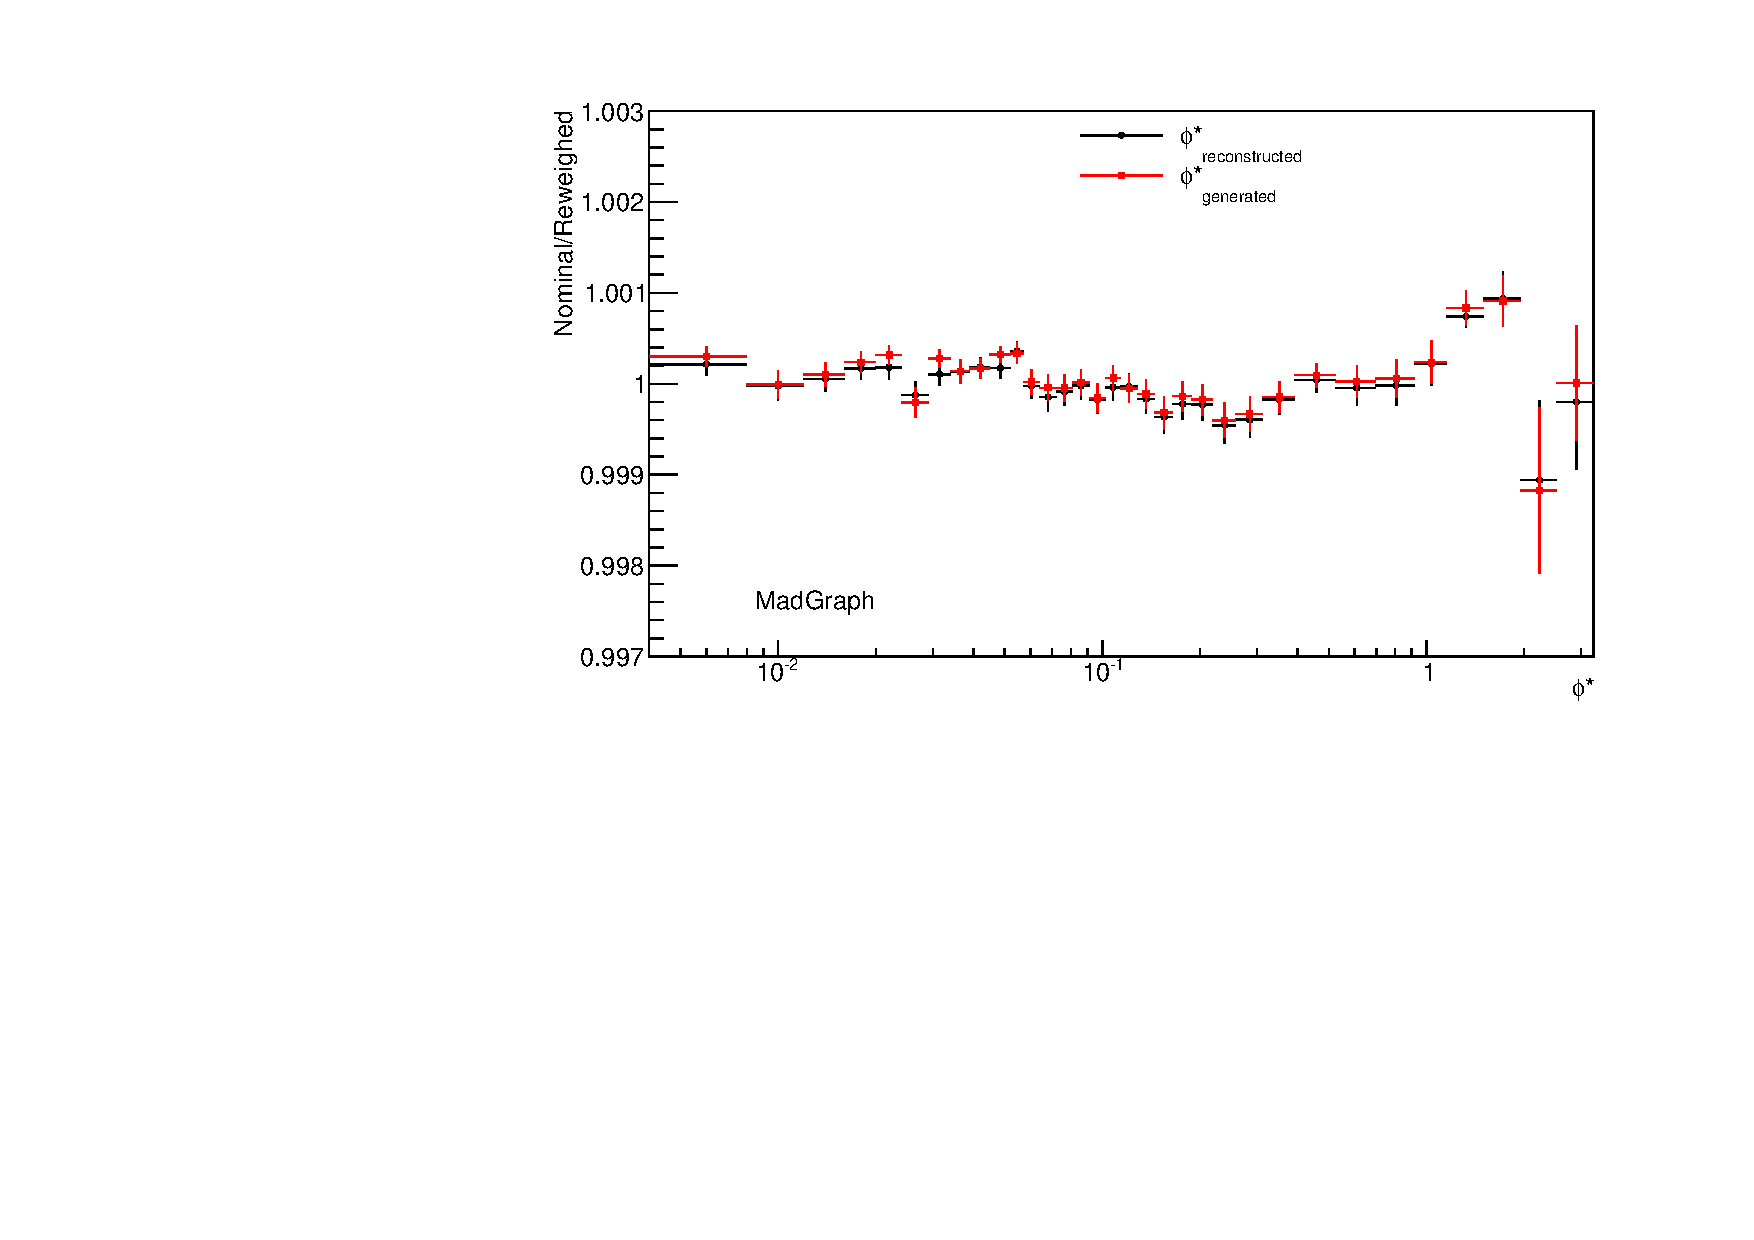
\includegraphics[width=\textwidth]{figures/ZMass_reweighed.pdf}
    \caption[
        The ratio of \phistar in \MADGRAPH before and after reweighting to
        remove the differnce in the \mee distribution between MC and data.
    ]{
        The ratio of \phistar in \MADGRAPH before and after reweighting to
        remove the difference in the \mee distribution between MC and data seen
        in \FIG~\ref{fig:z_mass}. The circular points are the ratio in the
        reconstructed quantity, while the square points are the ratio in the
        generated quantity. The uncertainties are binomial.
    }
    \label{fig:z_mass_reweighted}
\end{figure}

\TODO{Reweighting the \Z \pt plot?}

\section{Uncertainty Tables}

Tables summarizing the values of the various uncertainties as well as the total
uncertainty in each bin of \phistar for both the data and for the \MADGRAPH
signal MC sample are given below. The data tables,
\TABS~\ref{tab:sys_uncert_abs} and \ref{tab:sys_uncert_norm}, contain the
following columns:

\begin{description}[noitemsep]

    \item[\phistar Range:] \hfill \\
        The range of \phistar values included in the bin.

    \item[Total Uncertainty (Total):] \hfill \\
        The quadrature sum of the all of the uncertainties.

    \item[Statistical Uncertainty (Stat.):] \hfill \\
        The uncertainty due to the limited number of events in the data, as
        discussed in \SEC~\ref{ssec:stat_uncertainty}.

    \item[Total Systematic Uncertainty (Total Syst.):] \hfill \\
        The quadrature sum of all of the systematic uncertainties including,
        for the absolute distribution, the luminosity uncertainty of
        \LumiUncertainty.

    \item[Monte Carlo Statistical Uncertainty (MC Stat.):] \hfill \\
        The uncertainty due to the limited number of events in the MC samples,
        as discussed in \SEC~\ref{ssec:mc_stat_uncertainty}.

    \item[Pileup Uncertainty (Pileup):] \hfill \\
        The uncertainty due to the pileup reweighting, as discussed in
        \SEC~\ref{ssec:pileup_uncertainty}.

    \item[Background Subtraction Uncertainty (Bkg.):] \hfill \\
        The uncertainty due to background subtraction, as discussed in
        \SEC~\ref{ssec:background_subtraction_uncertainty}.

    \item[\pt Scale Uncertainty (\pt Scale):] \hfill \\
        The uncertainty due to \pt scale, as discussed in
        \SEC~\ref{ssec:pt_scale_uncertainty}.

    \item[Scale Factor Uncertainty (SF):] \hfill \\
        The uncertainty due to the scale factors, as discussed in
        \SEC~\ref{scale_factor_uncertainty}.

\end{description}

The MC tables, \TABS~\ref{tab:madgraph_uncert_abs}, \ref{tab:powheg_uncer_abs},
\ref{tab:madgraph_uncert_norm}, and \ref{tab:powheg_uncer_norm}, have the
following columns:

\begin{description}[noitemsep]

    \item[\phistar Range:] \hfill \\
        The range of \phistar values included in the bin.

    \item[Total Uncertainty (Total):] \hfill \\
        The quadrature sum of the all of the uncertainties.

    \item[Statistical Uncertainty (Stat.):] \hfill \\
        The uncertainty due to the limited number of events in the MC sample.

    \item[Parton Density Function (PDF):] \hfill \\
        The uncertainty due to choice of PDF used to generate the \POWHEG MC,
        as discussed in \SEC~\ref{ssec:pdf_uncertainties}.

    \item[Theoretical Cross Section Uncertainty (Cross Section):] \hfill \\
        The uncertainty in the theoretical cross section of the \MADGRAPH MC,
        as discussed in \SEC~\ref{ssec:pdf_uncertainties}.

    \item[Final State Radiation Uncertainty (FSR):] \hfill \\
        The uncertainty due to the modeling of FSR, as discussed in
        \SEC~\ref{ssec:fsr_uncertainties}.

\end{description}

% Absolute
\begin{table}
    \spacerows{1.05}
    \begin{center}
        \begin{tabular}{@{}l l l l l l l l l@{}}
            \toprule
            \phistar Range  &  Total  &  Stat.  &  Total Syst.  &  MC Stat.  &  Pileup  &  SF    &  \pt Scale  &  Bkg.  \\
            \midrule
            0.000--0.004    &  2.72   &  0.26   &  2.70         &  0.33      &  0.48    &  0.43  &  0.16       &  0.02  \\
            0.004--0.008    &  2.72   &  0.28   &  2.70         &  0.40      &  0.41    &  0.43  &  0.17       &  0.05  \\
            0.008--0.012    &  2.71   &  0.29   &  2.69         &  0.36      &  0.39    &  0.43  &  0.15       &  0.03  \\
            0.012--0.016    &  2.72   &  0.29   &  2.71         &  0.40      &  0.43    &  0.43  &  0.16       &  0.03  \\
            0.016--0.020    &  2.75   &  0.29   &  2.73         &  0.39      &  0.58    &  0.43  &  0.15       &  0.03  \\
            0.020--0.024    &  2.71   &  0.30   &  2.69         &  0.39      &  0.33    &  0.43  &  0.17       &  0.04  \\
            0.024--0.029    &  2.72   &  0.27   &  2.70         &  0.34      &  0.47    &  0.44  &  0.15       &  0.04  \\
            0.029--0.034    &  2.72   &  0.28   &  2.71         &  0.36      &  0.48    &  0.43  &  0.14       &  0.03  \\
            0.034--0.039    &  2.72   &  0.29   &  2.71         &  0.37      &  0.48    &  0.43  &  0.17       &  0.03  \\
            0.039--0.045    &  2.71   &  0.27   &  2.70         &  0.33      &  0.45    &  0.44  &  0.15       &  0.03  \\
            0.045--0.052    &  2.71   &  0.25   &  2.70         &  0.33      &  0.45    &  0.44  &  0.13       &  0.03  \\
            0.052--0.057    &  2.73   &  0.32   &  2.71         &  0.40      &  0.45    &  0.43  &  0.15       &  0.03  \\
            0.057--0.064    &  2.71   &  0.28   &  2.70         &  0.35      &  0.41    &  0.44  &  0.16       &  0.03  \\
            0.064--0.072    &  2.73   &  0.27   &  2.72         &  0.34      &  0.56    &  0.44  &  0.16       &  0.02  \\
            0.072--0.081    &  2.71   &  0.26   &  2.70         &  0.33      &  0.45    &  0.44  &  0.16       &  0.04  \\
            0.081--0.091    &  2.71   &  0.27   &  2.70         &  0.32      &  0.46    &  0.44  &  0.14       &  0.03  \\
            0.091--0.102    &  2.72   &  0.27   &  2.71         &  0.33      &  0.51    &  0.44  &  0.15       &  0.03  \\
            0.102--0.114    &  2.72   &  0.27   &  2.71         &  0.34      &  0.49    &  0.43  &  0.14       &  0.04  \\
            0.114--0.128    &  2.72   &  0.27   &  2.70         &  0.33      &  0.47    &  0.44  &  0.15       &  0.05  \\
            0.128--0.145    &  2.70   &  0.26   &  2.69         &  0.32      &  0.37    &  0.43  &  0.16       &  0.07  \\
            0.145--0.165    &  2.70   &  0.26   &  2.69         &  0.32      &  0.41    &  0.43  &  0.15       &  0.05  \\
            0.165--0.189    &  2.70   &  0.26   &  2.69         &  0.32      &  0.39    &  0.43  &  0.14       &  0.05  \\
            0.189--0.219    &  2.70   &  0.26   &  2.69         &  0.32      &  0.41    &  0.43  &  0.14       &  0.10  \\
            0.219--0.258    &  2.72   &  0.26   &  2.70         &  0.32      &  0.48    &  0.43  &  0.16       &  0.09  \\
            0.258--0.312    &  2.71   &  0.26   &  2.69         &  0.31      &  0.43    &  0.42  &  0.15       &  0.10  \\
            0.312--0.391    &  2.70   &  0.26   &  2.69         &  0.31      &  0.42    &  0.42  &  0.15       &  0.12  \\
            0.391--0.524    &  2.71   &  0.26   &  2.69         &  0.32      &  0.42    &  0.41  &  0.14       &  0.17  \\
            0.524--0.695    &  2.73   &  0.32   &  2.72         &  0.38      &  0.49    &  0.41  &  0.12       &  0.23  \\
            0.695--0.918    &  2.73   &  0.39   &  2.70         &  0.47      &  0.22    &  0.41  &  0.11       &  0.32  \\
            0.918--1.153    &  2.81   &  0.54   &  2.76         &  0.65      &  0.33    &  0.42  &  0.11       &  0.38  \\
            1.153--1.496    &  2.85   &  0.61   &  2.79         &  0.71      &  0.32    &  0.43  &  0.07       &  0.44  \\
            1.496--1.947    &  2.95   &  0.77   &  2.84         &  0.85      &  0.39    &  0.44  &  0.15       &  0.50  \\
            1.947--2.522    &  3.09   &  0.99   &  2.93         &  1.11      &  0.21    &  0.44  &  0.15       &  0.59  \\
            2.522--3.277    &  3.27   &  1.21   &  3.04         &  1.36      &  0.13    &  0.44  &  0.08       &  0.64  \\
            \bottomrule
        \end{tabular}
    \end{center}
    \caption[
        Fractional errors for the absolute cross section measurement
        made with data unfolded with \MADGRAPH.
    ]{
        Fractional errors (in \%) for the absolute cross section measurement
        made with data unfolded with \MADGRAPH. The total value and the total
        systematic value includes the uncertainty of 2.6\% due to luminosity.
    }
    \label{tab:sys_uncert_abs}
\end{table}

\begin{table}
    \spacerows{1.05}
    \begin{center}
        \begin{tabular}{@{}l l l l l@{}}
            \toprule
            \phistar Range & Total & Stat. & Cross Section & FSR \\
            \midrule
            0.000--0.004 & 3.32 & 0.26 & 3.30 & 0.27  \\
            0.004--0.008 & 3.32 & 0.27 & 3.30 & 0.27  \\
            0.008--0.012 & 3.32 & 0.27 & 3.30 & 0.27  \\
            0.012--0.016 & 3.32 & 0.27 & 3.30 & 0.27  \\
            0.016--0.020 & 3.32 & 0.27 & 3.30 & 0.27  \\
            0.020--0.024 & 3.32 & 0.28 & 3.30 & 0.27  \\
            0.024--0.029 & 3.32 & 0.25 & 3.30 & 0.27  \\
            0.029--0.034 & 3.32 & 0.26 & 3.30 & 0.28  \\
            0.034--0.039 & 3.32 & 0.27 & 3.30 & 0.28  \\
            0.039--0.045 & 3.32 & 0.25 & 3.30 & 0.28  \\
            0.045--0.052 & 3.32 & 0.25 & 3.30 & 0.29  \\
            0.052--0.057 & 3.33 & 0.30 & 3.30 & 0.29  \\
            0.057--0.064 & 3.32 & 0.27 & 3.30 & 0.29  \\
            0.064--0.072 & 3.32 & 0.26 & 3.30 & 0.29  \\
            0.072--0.081 & 3.32 & 0.26 & 3.30 & 0.30  \\
            0.081--0.091 & 3.32 & 0.26 & 3.30 & 0.30  \\
            0.091--0.102 & 3.32 & 0.27 & 3.30 & 0.30  \\
            0.102--0.114 & 3.33 & 0.27 & 3.30 & 0.31  \\
            0.114--0.128 & 3.33 & 0.27 & 3.30 & 0.31  \\
            0.128--0.145 & 3.33 & 0.27 & 3.30 & 0.32  \\
            0.145--0.165 & 3.33 & 0.27 & 3.30 & 0.32  \\
            0.165--0.189 & 3.33 & 0.27 & 3.30 & 0.32  \\
            0.189--0.219 & 3.33 & 0.27 & 3.30 & 0.32  \\
            0.219--0.258 & 3.33 & 0.27 & 3.30 & 0.32  \\
            0.258--0.312 & 3.33 & 0.27 & 3.30 & 0.32  \\
            0.312--0.391 & 3.33 & 0.28 & 3.30 & 0.32  \\
            0.391--0.524 & 3.33 & 0.28 & 3.30 & 0.33  \\
            0.524--0.695 & 3.33 & 0.34 & 3.30 & 0.32  \\
            0.695--0.918 & 3.34 & 0.42 & 3.30 & 0.32  \\
            0.918--1.153 & 3.36 & 0.57 & 3.30 & 0.33  \\
            1.153--1.496 & 3.38 & 0.65 & 3.30 & 0.33  \\
            1.496--1.947 & 3.41 & 0.80 & 3.30 & 0.33  \\
            1.947--2.522 & 3.47 & 1.02 & 3.30 & 0.34  \\
            2.522--3.277 & 3.55 & 1.26 & 3.30 & 0.34  \\
            \bottomrule
        \end{tabular}
    \end{center}
    \caption{
        Fractional errors (in \%) for the absolute cross section from the
        \MADGRAPH MC sample.
    }
    \label{tab:madgraph_uncert_abs}
\end{table}

\begin{table}
    \spacerows{1.05}
    \begin{center}
        \begin{tabular}{@{}l l l l l@{}}
            \toprule
            \phistar Range & Total & Stat. & PDF & FSR \\
            \midrule
            0.000--0.004 & 2.72 & 0.62 & 2.63 & 0.27  \\
            0.004--0.008 & 2.71 & 0.62 & 2.63 & 0.27  \\
            0.008--0.012 & 2.68 & 0.63 & 2.59 & 0.27  \\
            0.012--0.016 & 2.75 & 0.63 & 2.66 & 0.28  \\
            0.016--0.020 & 2.71 & 0.64 & 2.62 & 0.28  \\
            0.020--0.024 & 2.74 & 0.64 & 2.65 & 0.28  \\
            0.024--0.029 & 2.73 & 0.58 & 2.65 & 0.27  \\
            0.029--0.034 & 2.70 & 0.59 & 2.62 & 0.27  \\
            0.034--0.039 & 2.72 & 0.61 & 2.64 & 0.28  \\
            0.039--0.045 & 2.69 & 0.57 & 2.61 & 0.28  \\
            0.045--0.052 & 2.70 & 0.54 & 2.63 & 0.28  \\
            0.052--0.057 & 2.75 & 0.67 & 2.66 & 0.28  \\
            0.057--0.064 & 2.74 & 0.59 & 2.66 & 0.29  \\
            0.064--0.072 & 2.75 & 0.57 & 2.67 & 0.29  \\
            0.072--0.081 & 2.71 & 0.57 & 2.63 & 0.30  \\
            0.081--0.091 & 2.70 & 0.57 & 2.62 & 0.30  \\
            0.091--0.102 & 2.75 & 0.58 & 2.67 & 0.30  \\
            0.102--0.114 & 2.72 & 0.60 & 2.63 & 0.31  \\
            0.114--0.128 & 2.72 & 0.60 & 2.64 & 0.32  \\
            0.128--0.145 & 2.71 & 0.59 & 2.63 & 0.31  \\
            0.145--0.165 & 2.71 & 0.60 & 2.62 & 0.31  \\
            0.165--0.189 & 2.73 & 0.61 & 2.65 & 0.31  \\
            0.189--0.219 & 2.73 & 0.61 & 2.64 & 0.33  \\
            0.219--0.258 & 2.67 & 0.61 & 2.58 & 0.32  \\
            0.258--0.312 & 2.66 & 0.61 & 2.57 & 0.32  \\
            0.312--0.391 & 2.61 & 0.62 & 2.52 & 0.33  \\
            0.391--0.524 & 2.57 & 0.63 & 2.47 & 0.32  \\
            0.524--0.695 & 2.65 & 0.78 & 2.51 & 0.32  \\
            0.695--0.918 & 2.65 & 0.97 & 2.44 & 0.33  \\
            0.918--1.153 & 2.79 & 1.34 & 2.42 & 0.35  \\
            1.153--1.496 & 2.91 & 1.57 & 2.43 & 0.33  \\
            1.496--1.947 & 3.20 & 2.00 & 2.47 & 0.33  \\
            1.947--2.522 & 3.62 & 2.55 & 2.55 & 0.35  \\
            2.522--3.277 & 4.03 & 3.04 & 2.62 & 0.33  \\
            \bottomrule
        \end{tabular}
    \end{center}
    \caption{
        Total errors (in \%) for the absolute cross section from the \POWHEG
        MC sample.
    }
    \label{tab:powheg_uncert_abs}
\end{table}


% Normalized
\begin{table}
    \spacerows{1.05}
    \begin{center}
        \begin{tabular}{@{}l l l l l l l l l@{}}
            \toprule
            \phistar Range  &  Total  &  Stat.  &  Total Syst.  &  MC Stat.  &  Pileup  &  SF    &  \pt Scale  &  Bkg.  \\
            \midrule
            0.000--0.004    &  0.43   &  0.26   &  0.34         &  0.33      &  0.04    &  0.07  &  0.01       &  0.05  \\
            0.004--0.008    &  0.50   &  0.28   &  0.41         &  0.40      &  0.03    &  0.07  &  0.02       &  0.05  \\
            0.008--0.012    &  0.47   &  0.29   &  0.37         &  0.36      &  0.02    &  0.07  &  0.00       &  0.04  \\
            0.012--0.016    &  0.50   &  0.29   &  0.41         &  0.40      &  0.02    &  0.07  &  0.01       &  0.04  \\
            0.016--0.020    &  0.51   &  0.29   &  0.42         &  0.39      &  0.14    &  0.07  &  0.00       &  0.04  \\
            0.020--0.024    &  0.51   &  0.30   &  0.41         &  0.39      &  0.10    &  0.07  &  0.02       &  0.04  \\
            0.024--0.029    &  0.44   &  0.27   &  0.35         &  0.33      &  0.03    &  0.07  &  0.01       &  0.04  \\
            0.029--0.034    &  0.46   &  0.28   &  0.37         &  0.36      &  0.04    &  0.07  &  0.01       &  0.04  \\
            0.034--0.039    &  0.48   &  0.28   &  0.38         &  0.37      &  0.04    &  0.06  &  0.02       &  0.04  \\
            0.039--0.045    &  0.43   &  0.27   &  0.34         &  0.33      &  0.01    &  0.06  &  0.00       &  0.05  \\
            0.045--0.052    &  0.42   &  0.25   &  0.34         &  0.33      &  0.01    &  0.06  &  0.00       &  0.04  \\
            0.052--0.057    &  0.52   &  0.32   &  0.40         &  0.40      &  0.01    &  0.05  &  0.01       &  0.05  \\
            0.057--0.064    &  0.45   &  0.28   &  0.35         &  0.35      &  0.02    &  0.05  &  0.01       &  0.04  \\
            0.064--0.072    &  0.45   &  0.27   &  0.36         &  0.33      &  0.11    &  0.05  &  0.01       &  0.04  \\
            0.072--0.081    &  0.43   &  0.26   &  0.34         &  0.33      &  0.01    &  0.04  &  0.02       &  0.04  \\
            0.081--0.091    &  0.42   &  0.26   &  0.33         &  0.32      &  0.02    &  0.03  &  0.00       &  0.04  \\
            0.091--0.102    &  0.43   &  0.27   &  0.34         &  0.33      &  0.07    &  0.03  &  0.00       &  0.04  \\
            0.102--0.114    &  0.44   &  0.27   &  0.35         &  0.34      &  0.05    &  0.02  &  0.00       &  0.04  \\
            0.114--0.128    &  0.43   &  0.27   &  0.33         &  0.33      &  0.03    &  0.03  &  0.01       &  0.03  \\
            0.128--0.145    &  0.43   &  0.26   &  0.34         &  0.32      &  0.10    &  0.03  &  0.01       &  0.03  \\
            0.145--0.165    &  0.42   &  0.26   &  0.33         &  0.32      &  0.04    &  0.04  &  0.00       &  0.03  \\
            0.165--0.189    &  0.42   &  0.26   &  0.33         &  0.32      &  0.05    &  0.05  &  0.02       &  0.03  \\
            0.189--0.219    &  0.43   &  0.26   &  0.33         &  0.32      &  0.04    &  0.06  &  0.01       &  0.06  \\
            0.219--0.258    &  0.42   &  0.26   &  0.33         &  0.32      &  0.04    &  0.08  &  0.01       &  0.04  \\
            0.258--0.312    &  0.42   &  0.26   &  0.33         &  0.31      &  0.03    &  0.10  &  0.01       &  0.05  \\
            0.312--0.391    &  0.43   &  0.26   &  0.35         &  0.31      &  0.04    &  0.13  &  0.00       &  0.07  \\
            0.391--0.524    &  0.45   &  0.26   &  0.37         &  0.31      &  0.00    &  0.15  &  0.00       &  0.12  \\
            0.524--0.695    &  0.56   &  0.32   &  0.46         &  0.38      &  0.04    &  0.19  &  0.02       &  0.18  \\
            0.695--0.918    &  0.73   &  0.39   &  0.62         &  0.47      &  0.20    &  0.23  &  0.01       &  0.27  \\
            0.918--1.153    &  0.95   &  0.53   &  0.79         &  0.65      &  0.10    &  0.27  &  0.05       &  0.33  \\
            1.153--1.496    &  1.07   &  0.61   &  0.87         &  0.71      &  0.08    &  0.31  &  0.06       &  0.39  \\
            1.496--1.947    &  1.27   &  0.77   &  1.02         &  0.85      &  0.00    &  0.33  &  0.05       &  0.45  \\
            1.947--2.522    &  1.73   &  0.98   &  1.43         &  1.10      &  0.64    &  0.35  &  0.00       &  0.54  \\
            2.522--3.277    &  2.02   &  1.21   &  1.62         &  1.36      &  0.56    &  0.34  &  0.10       &  0.59  \\
            \bottomrule
        \end{tabular}
    \end{center}
    \caption[
        The uncertainties for the normalized cross section measurement made
        with data unfolded with \MADGRAPH.
    ]{
        The uncertainties (in \%) for the normalized cross section measurement
        made with data unfolded with \MADGRAPH.
    }
    \label{tab:sys_uncert_norm}
\end{table}

\begin{table}
    \spacerows{1.05}
    \begin{center}
        \begin{tabular}{@{}l l l l@{}}
            \toprule
            \phistar Range & Total & Stat. & FSR \\
            \midrule
            0.000--0.004 & 0.27 & 0.26 & 0.03  \\
            0.004--0.008 & 0.27 & 0.27 & 0.03  \\
            0.008--0.012 & 0.27 & 0.27 & 0.03  \\
            0.012--0.016 & 0.27 & 0.27 & 0.03  \\
            0.016--0.020 & 0.27 & 0.27 & 0.03  \\
            0.020--0.024 & 0.28 & 0.28 & 0.02  \\
            0.024--0.029 & 0.26 & 0.25 & 0.03  \\
            0.029--0.034 & 0.26 & 0.26 & 0.02  \\
            0.034--0.039 & 0.27 & 0.27 & 0.02  \\
            0.039--0.045 & 0.25 & 0.25 & 0.02  \\
            0.045--0.052 & 0.25 & 0.25 & 0.01  \\
            0.052--0.057 & 0.30 & 0.30 & 0.01  \\
            0.057--0.064 & 0.27 & 0.27 & 0.01  \\
            0.064--0.072 & 0.26 & 0.26 & 0.00  \\
            0.072--0.081 & 0.26 & 0.26 & 0.00  \\
            0.081--0.091 & 0.26 & 0.26 & 0.01  \\
            0.091--0.102 & 0.27 & 0.27 & 0.01  \\
            0.102--0.114 & 0.27 & 0.27 & 0.01  \\
            0.114--0.128 & 0.27 & 0.27 & 0.02  \\
            0.128--0.145 & 0.27 & 0.27 & 0.02  \\
            0.145--0.165 & 0.27 & 0.27 & 0.02  \\
            0.165--0.189 & 0.27 & 0.27 & 0.02  \\
            0.189--0.219 & 0.27 & 0.27 & 0.02  \\
            0.219--0.258 & 0.28 & 0.27 & 0.03  \\
            0.258--0.312 & 0.28 & 0.27 & 0.03  \\
            0.312--0.391 & 0.28 & 0.28 & 0.03  \\
            0.391--0.524 & 0.28 & 0.28 & 0.03  \\
            0.524--0.695 & 0.34 & 0.34 & 0.03  \\
            0.695--0.918 & 0.42 & 0.42 & 0.03  \\
            0.918--1.153 & 0.57 & 0.57 & 0.03  \\
            1.153--1.496 & 0.65 & 0.65 & 0.03  \\
            1.496--1.947 & 0.80 & 0.80 & 0.03  \\
            1.947--2.522 & 1.02 & 1.02 & 0.04  \\
            2.522--3.277 & 1.26 & 1.26 & 0.04  \\
            \bottomrule
        \end{tabular}
    \end{center}
    \caption{
        Total errors (in \%) for the normalized absolute cross section from the
        \MADGRAPH MC sample.
    }
    \label{tab:madgraph_uncert_norm}
\end{table}

\begin{table}
    \spacerows{1.05}
    \begin{center}
        \begin{tabular}{@{}l l l l l@{}}
            \toprule
            \phistar Range & Total & Stat. & PDF & FSR \\
            \midrule
            0.000-0.004 & 0.63 & 0.62 & 0.13 & 0.02  \\
            0.004-0.008 & 0.63 & 0.62 & 0.13 & 0.02  \\
            0.008-0.012 & 0.65 & 0.63 & 0.15 & 0.02  \\
            0.012-0.016 & 0.65 & 0.63 & 0.15 & 0.02  \\
            0.016-0.020 & 0.65 & 0.64 & 0.13 & 0.02  \\
            0.020-0.024 & 0.65 & 0.64 & 0.13 & 0.02  \\
            0.024-0.029 & 0.60 & 0.58 & 0.12 & 0.03  \\
            0.029-0.034 & 0.60 & 0.59 & 0.09 & 0.02  \\
            0.034-0.039 & 0.62 & 0.61 & 0.10 & 0.01  \\
            0.039-0.045 & 0.58 & 0.57 & 0.09 & 0.02  \\
            0.045-0.052 & 0.55 & 0.54 & 0.08 & 0.02  \\
            0.052-0.057 & 0.68 & 0.67 & 0.11 & 0.02  \\
            0.057-0.064 & 0.60 & 0.59 & 0.11 & 0.01  \\
            0.064-0.072 & 0.59 & 0.57 & 0.14 & 0.01  \\
            0.072-0.081 & 0.57 & 0.57 & 0.06 & 0.00  \\
            0.081-0.091 & 0.57 & 0.57 & 0.04 & 0.00  \\
            0.091-0.102 & 0.61 & 0.58 & 0.18 & 0.00  \\
            0.102-0.114 & 0.60 & 0.60 & 0.09 & 0.01  \\
            0.114-0.128 & 0.61 & 0.60 & 0.12 & 0.02  \\
            0.128-0.145 & 0.60 & 0.59 & 0.11 & 0.02  \\
            0.145-0.165 & 0.62 & 0.60 & 0.16 & 0.02  \\
            0.165-0.189 & 0.64 & 0.61 & 0.19 & 0.01  \\
            0.189-0.219 & 0.65 & 0.61 & 0.23 & 0.03  \\
            0.219-0.258 & 0.63 & 0.61 & 0.16 & 0.02  \\
            0.258-0.312 & 0.63 & 0.61 & 0.15 & 0.03  \\
            0.312-0.391 & 0.65 & 0.62 & 0.20 & 0.03  \\
            0.391-0.524 & 0.67 & 0.63 & 0.24 & 0.03  \\
            0.524-0.695 & 0.81 & 0.78 & 0.23 & 0.02  \\
            0.695-0.918 & 1.05 & 0.97 & 0.41 & 0.03  \\
            0.918-1.153 & 1.47 & 1.34 & 0.60 & 0.05  \\
            1.153-1.496 & 1.74 & 1.57 & 0.76 & 0.03  \\
            1.496-1.947 & 2.15 & 2.00 & 0.78 & 0.04  \\
            1.947-2.522 & 2.76 & 2.55 & 1.07 & 0.06  \\
            2.522-3.277 & 3.26 & 3.04 & 1.17 & 0.03  \\
            \bottomrule
        \end{tabular}
    \end{center}
    \caption{
        Total errors (in \%) for the normalized cross section from the
        \POWHEG MC sample.
    }
    \label{tab:powheg_uncert_norm}
\end{table}

